\vspace*{-1mm}
In Chapter~\ref{Ch:CC_noise_theory} the theoretical model for the transverse emittance growth caused by amplitude and phase noise in a $\CC$ was discussed. On September 5, 2018, a dedicated experiment was conducted in the SPS to benchmark this model against experimental data and confirm the analytical predictions. In particular, the idea was to inject artificial noise in the $\CC$ RF system and compare the measured emittance growth rates with the the theoretically computed ones. In this chapter the measurement results from the SPS are presented and discussed. The work published in Ref.~\cite{Triantafyllou:2021khx} is the basis of this chapter.


Section ... describes the machine setup and the beam configuration for the emittance growth measurements. This includes a summary of the preparatory studies conducted in the previous years. In Section ...


\section{Experimental configuration and procedure}\label{sec:exp_setup_2018}
This section gives an overview of the experimental setup and the procedure that was followed. First, it briefly discusses the preparatory studies that were performed during 2012-2017~\cite{Calaga:1451286, Alekou_CC_coast_prep_2016, Antoniou:2649815}, explaining the choice of the intensity and energy values for which the emittance growth measurements were conducted. Furthermore, it presents in detail the rest of the beam and machine conditions during the experiment. Last, the experimental procedure is explained.

%\normalsize{\textbf{Preparatory experimental studies}}\\
\subsection{Preparatory experimental studies}
For studying the long-term emittance evolution a special mode of operation was set up in the SPS which is called "coast" (in other machines, it is referred to as storage ring mode) with bunched beams. In this mode, the bunches circulate in the machine at constant energy for long periods, from a few minutes up to several hours, similar to the HL-LHC case.\setlength{\parskip}{2ex} %set it manually here, as for some reason it was not displayed properly in the pdf.

To make sure that the SPS can be used as a testbed for the emittance growth studies with $\CC$s an extensive preparatory campaign was carried out through 2012-2017~\cite{Calaga:1451286, Alekou_CC_coast_prep_2016, Antoniou:2649815}. The primary concern was the emittance growth that was observed in the machine from other sources than injected noise and will be referred to as the natural emittance growth in this thesis. The natural emittance growth needs to be well characterized and be kept sufficiently small in order to distinguish and understand the contribution from the $\CC$ noise. 

From these studies, it was concluded that the optimal coast setup is at high energies, with low chromaticity and bunches of low intensity as it minimises the natural emittance growth~\cite{Antoniou:2649815}. The highest energy for which the SPS could operate in "coast" was 270\,GeV and thus the experiments were performed at this energy. That limitation was introduced due to the rms power deposited in its magnets when operating at high energy for long period of time. Moreover, as the natural emittance growth was found to be a single bunch effect four bunches were used. That choice was made to reduce the statistical uncertainty of the measurements but not to increase the beam intensity.

%\normalsize{\textbf{Machine and beam configuration}}\\
\subsection{Machine and beam configuration}
During the experiment the Landau octupoles were switched off. Nevetherless, a residual non-linearity was present in the machine mainly due to multipole components in the dipole magnets~\cite{Carlà:2664976, Alekou:2640326}. The transverse feedback system was also switched off. Unfortunately, no measurements of chromaticity are available from the day of the experiment. However it was ensured that the chromaticity was corrected to small positive values. 

Last, only one $\CC$, $\CC 2$, was used for simplicity and it operated at 1\,MV. This value was validated with the HT monitor (post-processing procedure desribed in Chapter~\ref{Ch:CC_set_up}). Unfortunately, only one beam based measurement of the $\CC$ voltage is available whcih is displayed in Fig.~\ref{fig:crabbing_sin_fit_MD5}. It is clear that the measured value of voltage amplitude, $\VCC$ = 0.99 $\pm$ 0.04\,MV , is in good agreement with the requested one. It should be noted, that due to the beam energy of 270\,GeV the crabbing is less visible than the example discussed in Chapter~\ref{Ch:CC_set_up} (see Fig.~\ref{fig:crabbing_sin_fit_MD2}) for 26\,GeV. Therefore, here the part of the signal that is used for the fit is the one for which the normalised sum signal (blck dashed line) is above 0.2 (instead of 0.4 that was the condition for the case of 26\,GeV)

\begin{figure}[!h]
   \centering         
   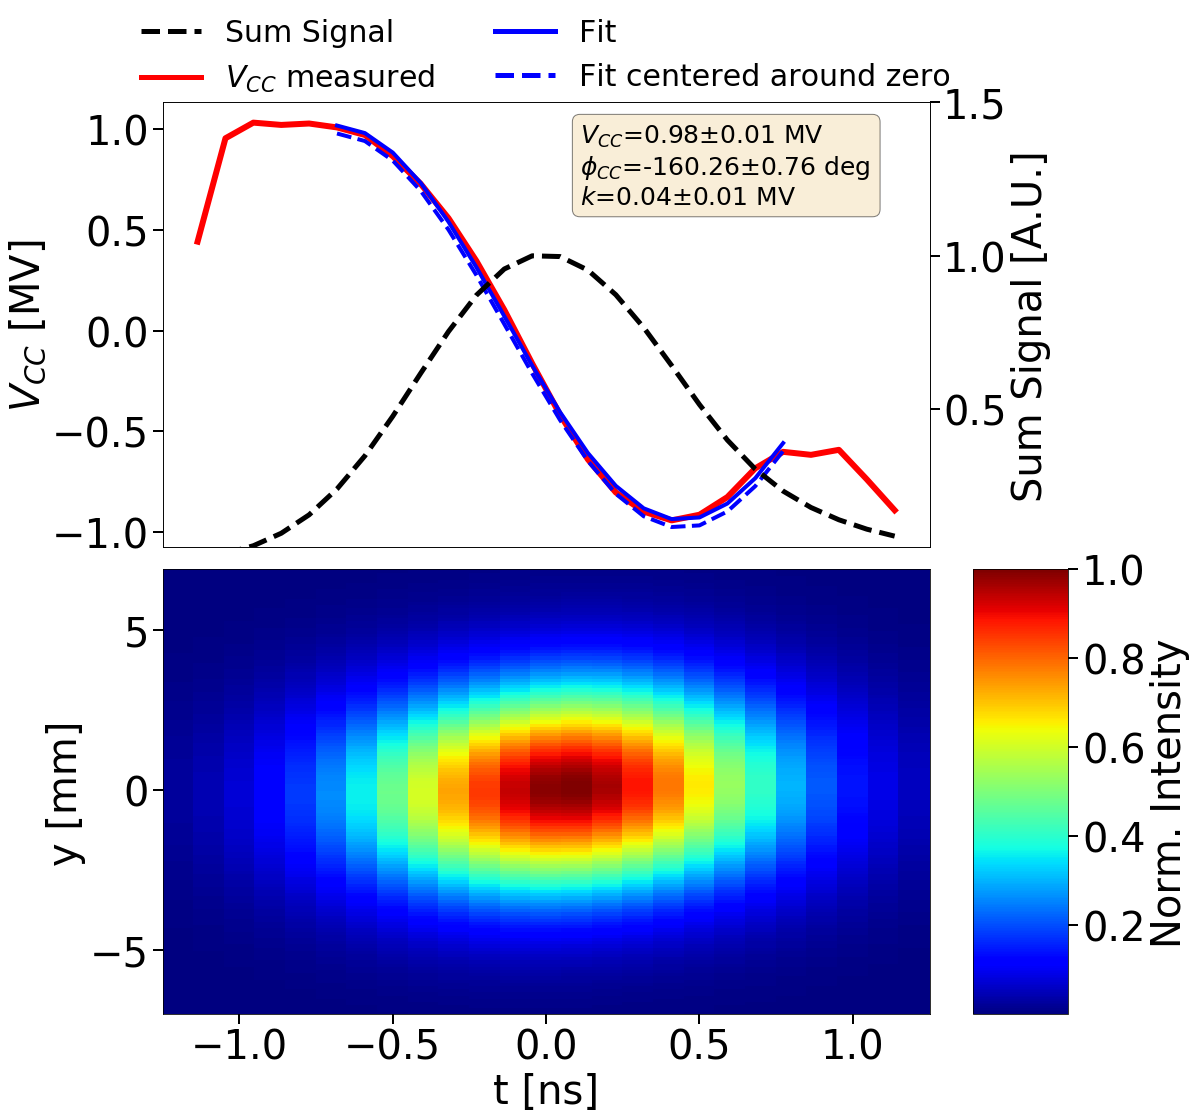
\includegraphics[width=0.7\textwidth]{images/Ch5/HT_VCC_callibration_20180905_135033_sin_fit_fixed_freq.png}
       \caption{Demonstration of the sinusoidal fit on the HT monitor reading in order to obtain the CC parameters as described in Section~\ref{sec:CC_voltage_meas}. The fit results, are given in the yellow box. The measured voltage amplitude, $V_{CC}$, was found to be 0.99\,MV while its uncertainty, $\Delta V_{CC}$, was measured at 0.04\,MV. The measured voltage value agrees well with the requested value of 1\,MV.}
       \label{fig:crabbing_sin_fit_MD5}
\end{figure}


The main machine and beam parameters used for the emittance growth measurements in 2018 are listed in Table~\ref{tab:machine_beam_param_2018}. % the parameters shown are the relatives one for Eq.(3.1) and (3.2) --> theoretical formulas for the emittance growht.


\begin{table}[!hbt]
	\begin{minipage}{\textwidth}
      \begin{centering}
   \caption{Main machine and beam parameters for the emittance growth studies with CCs in SPS in 2018.}
	\begin{tabu} to \textwidth {X[c,m] X[0.5c,m] X[0.5c,m] X[0.01c,m]}
		&&& \\[-6mm]
		\toprule \toprule
		\multicolumn{2}{l}{\textbf{Parameter}} &
		\multicolumn{2}{c}{\textbf{Value}} \\
		\bottomrule
      \multicolumn{2}{l}{Beam energy, $\symE$} & \multicolumn{2}{c}{270\,GeV} \\
      \multicolumn{2}{l}{Revolution frequency, $\frev$}  & \multicolumn{2}{c}{43.375\,kHz} \\
      \multicolumn{2}{l}{Main RF voltage / frequency,  $\VRF$ / $\fRF$}  & \multicolumn{2}{c}{3.8\,MV / 200.39\,MHz} \\ %200.3945
      \multicolumn{2}{l}{Horizontal / Vertical betatron tune, $\Qx$ / $\Qy$}  & \multicolumn{2}{c}{26.13 / 26.18} \\
      \multicolumn{2}{l}{Horizontal / Vertical first order chromaticity, $\Qpx$ / $\Qpy$}  & \multicolumn{2}{c}{ $\sim$ 1.0 / $\sim$ 1.0} \\
      \multicolumn{2}{l}{Synchrotron tune, $\Qs$}  & \multicolumn{2}{c}{0.0051} \\
      \multicolumn{2}{l}{$\CC 2$ voltage / frequency, $\VCC$ / $\fCC$}  & \multicolumn{2}{c}{1\,MV / 400.78\,MHz} \\
      \multicolumn{2}{l}{Number of protons per bunch, $\Nb$} & \multicolumn{2}{c}{3 $\times 10^{10}$ p/b$^\ast$} \\
      \multicolumn{2}{l}{Number of bunches}  & \multicolumn{2}{c}{4} \\
      \multicolumn{2}{l}{Bunch spacing}  & \multicolumn{2}{c}{524\,ns} \\
      \multicolumn{2}{l}{Rms bunch length, $\sigmat$}  & \multicolumn{2}{c}{1.8 \,ns$^\ast$}\\
      \multicolumn{2}{l}{Horizontal / Vertical normalised emittance, $\emitx$ / $\emity$}  & \multicolumn{2}{c}{2\,$\mathrm{\mu m}$ / 2\,$\mathrm{\mu m^\ast}$}\\
      \multicolumn{2}{l}{Horizontal / Vertical rms tune spread, $\Dqxrms$ / $\Dqyrms$}  & \multicolumn{2}{c}{2\,ns / 2\,ns$^\dagger$}\\
      \bottomrule
	\end{tabu}
   \label{tab:machine_beam_param_2018}
   \end{centering} \footnotesize{$^\ast$ The value correspond to the requested intial value at the start of each coast. The measured evolution of the parameter through the experiment is presented in the Sections~\ref{sec:emit_growth_meas_2018} and~\ref{sec:bunch_length_intensity_meas_2018}.\\$^\dagger$ Here the rms betatron tune spread includes only the contribution from the amplitude detuning introduced by the multiple components in the SPS dipole magnets. The calulcations for the listed values can be found in Appendix~\ref{app:detuning_with_amplitude}.}
   \end{minipage}
\end{table}


%\normalsize{\textbf{Experimental procedure}}\\
\subsection{Experimental procedure}\label{sec:experimental_procedure_2018}
The experiment took place on September 5, 2018, and was given a total time window of about 16 hours (start:$\sim$10:30, end:$\sim$17:00). In order to characterize the CC noise induced emittance growth, different levels of controlled noise were injected into its LLRF system and the bunch evolution was recorded for about 20-40 minutes (for each noise setting). The experiment was conducted over three coasts, since a new beam was injected every time the quality of the beam was seen to be degraded e.g. very large beam size. In the following, the diffrent noise settings will be denoted as "Coast$N$-Setting$M$", where $N$ stands for the coast number and $M$ for the different noise levels applied in each coast in chronological order. After the experiment, the measured growth rates would be compared with the theoretically expected values from the model described in Chapter~\ref{Ch:CC_noise_theory}.
%The dedicated experiment to study the emittance growth induced by noise in the $\CC$ RF sytsem took place on September 5, 2018, and was given a total time window of about 16 hours (start:$\sim$10:30, end:$\sim$17:00).

\section{Injected RF noise}\label{sec:injected_RF_noise}
The noise injected in the $\CC$ RF system was a mixture of amplitude and phase noise up to 10\,kHz, overlapping and primarily exciting the first betatron sideband at $\sim 8$\,kHz. The phase noise was always dominant. The noise levels were measured with a spectrum analyzer E5052B~\cite{E5052B_insight} and are expressed as $10\log_{10}\mathcal{L}(f)$\,[dBc/Hz]. The relation between the measrued noise levels and the PSDs in Eq.~\eqref{eq:dey_an} and Eq.~\eqref{eq:dey_pn} is given by $S_\Delta = 2\mathcal{L}(f)$, with $S_{\Delta A}$ in\,1/Hz and $S_{\Delta \phi}$ in $\mathrm{rad^2/Hz}$. This relation is extensivly discussed in Appendix~\ref{ch:app_B} and specifically in~\ref{app:Measured_noise}}. Figure~\ref{fig:example_PN_and_AN_coast1_setting2} displays an example measurement of amplitude (left) and phase (right) noise acquired during the experiment.

 % Loaction for creating the figure: /eos/user/n/natriant/2018/CC_MD_2018_summary/measured_psd
 \begin{figure}[!ht]
   \centering
   \begin{subfigure}[t]{0.45\textwidth}
       \centering
       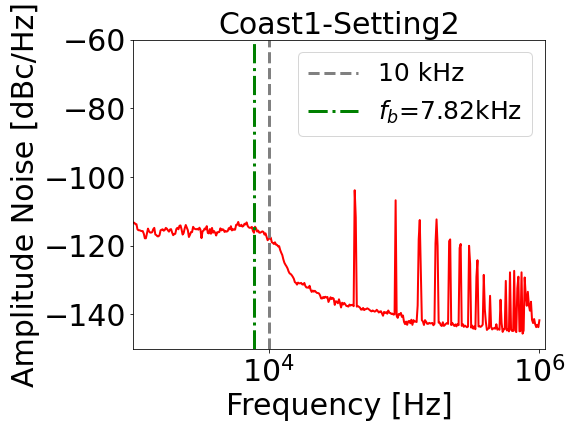
\includegraphics[width=1\textwidth]{images/Ch5/Measured_spectrum_MD5_Coast1-Setting2-AN.csv_no_psd.png}
       %\caption{$y=\sin(2 \pi f t),\ f=50$ Hz}
       %\label{fig:add_label_here}
   \end{subfigure}
   \hfill
   \begin{subfigure}[t]{0.45\textwidth}
       \centering
       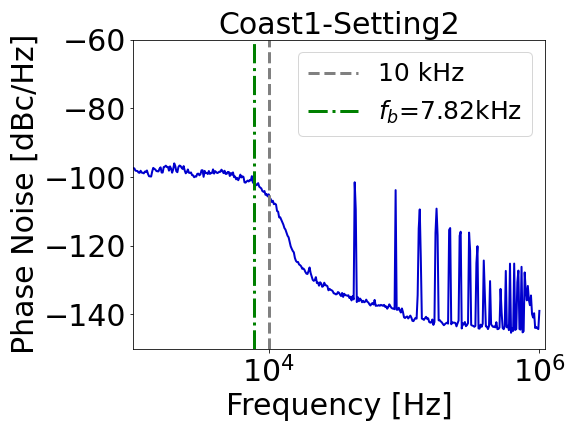
\includegraphics[width=1\textwidth]{images/Ch5/Measured_spectrum_MD5_Coast1-Setting2-PN.csv_no_psd.png}
       %\caption{Discrete Fourier transform}
       %\label{fig:add_label_here}
   \end{subfigure}
   \hfill
    \caption{Example amplitude (left) and phase (right) noise spectra measured with a spectrum analyzer E5052B~\cite{E5052B_insight} during the emittance growth studies with CCs in SPS. The noise spreads-out up to 10\,kHz (grey dashed line) overlapping the first betatron sideband at $\sim$8\,kHz (green dashed line). The spikes at high frequencies correspond to the harmonics of the revolution frequency and are a result of the bunch crossing.} % bunch passage
    \label{fig:example_PN_and_AN_coast1_setting2}
\end{figure}

\subsubsection*{PSD values of interest}
As already discussed in Chapter~\ref{Ch:CC_noise_theory} the noise induced emittance growth depends on the noise power at the beteatron and synchrobetatron sidebands for the phase and amplitude noise respectively (see Eq.~\eqref{eq:dey_pn} and Eq.~\eqref{eq:dey_an}). Therefore, the noise power values of interest for this thesis are the ones at the first betatron $f_b = 0.18 \times \frev$ = 7.82\,kHz and at the synchrobetatron sidebands at $f_b \pm \Qs \times \frev  = f_b \pm  \sim 220$\,kHz. 


However, it can be clearly seen from Fig.~\ref{fig:example_PN_and_AN_coast1_setting2} that the measured noise spectra are noisy: random changes in amplitude are observed from point to point within the signal. To this end, the PSD value at the first betatron sideband, $f_b$, is determined as the average of the PSD values over a frequency range of $\pm$ 500\,Hz around it. The spread of the values is also determined as the standard deviation over that range. In the following, it is assumed for simplicity that the PSD at the synchrobetatron sidebands equals the PSD at the first betaton sideband as they lie very close to each other. At this point, it should be mentioned that the validity of these assumptions was tested with numerical simulations including th measured spectra (Chapter~\ref{Ch:investigating_discrepancy}).

The emittance growth measurements were performed with seven different noise levels which are listed in Table~\ref{tab:noise_settings_2018}. 
% Script for computing the values: /eos/user/n/natriant/2018/CC_MD_2018_summary/measured_psd/job001_cmpt_psd_at_fb.ipynb
% The resulted pickle file can be found at: /eos/user/n/natriant/2018/CC_MD_2018_summary/measured_psd/output
\begin{table}[!hbt]
	\centering
   \caption{Phase and amplitude noise levels injected in the CC RF system for the emittance growth studies of 2018. The listed values correspond to the average PSD values over a frequency range of $\pm$ 500\,Hz around the first betatron sideband, $f_b$.}
	\begin{tabu} to \textwidth { X[c,m] X[c,m] X[c,m] X[c,m] }
		&&& \\[-6mm]
		\toprule \toprule
		\multicolumn{2}{l}{} &
		\multicolumn{2}{c}{$\mathbf{10\,\boldsymbol{\log}_{10} \mathcal{L}(f)}$ \textbf{[dBc/Hz]}} \\
		\bottomrule
      \multicolumn{2}{l}{} & 	\multicolumn{1}{c}{\textbf{Phase noise}} & \multicolumn{1}{c}{\textbf{Amplitude noise}} \\
      \midrule
      \multicolumn{2}{l}{Coast1-Setting1}  & \multicolumn{1}{c}{-122.6 $\pm 0.6$} & \multicolumn{1}{c}{-128.1 $\pm$ 0.6} \\
      
      \multicolumn{2}{l}{Coast1-Setting2}  & \multicolumn{1}{c}{-101.4 $\pm$ 0.8} & \multicolumn{1}{c}{-115.2 $\pm$ 0.6} \\

      \multicolumn{2}{l}{Coast2-Setting1}  & \multicolumn{1}{c}{-115.0 $\pm$ 0.8} & \multicolumn{1}{c}{-124.1 $\pm$ 0.5} \\

      \multicolumn{2}{l}{Coast2-Setting2}  & \multicolumn{1}{c}{-111.4 $\pm$ 0.6} & \multicolumn{1}{c}{-115.7 $\pm$ 0.4} \\ 

      \multicolumn{2}{l}{Coast3-Setting1}  & \multicolumn{1}{c}{-110.9 $\pm$ 0.9} & \multicolumn{1}{c}{-116.9 $\pm$ 0.4} \\

      \multicolumn{2}{l}{Coast3-Setting2} & \multicolumn{1}{c}{-106.4 $\pm$ 0.3} & \multicolumn{1}{c}{-112.9 $\pm$ 0.6} \\

      \multicolumn{2}{l}{Coast3-Setting3} & \multicolumn{1}{c}{-101.4 $\pm$ 0.7}  & \multicolumn{1}{c}{-106.9 $\pm$ 0.5} \\
      \arrayrulecolor{black}\bottomrule
 
	\end{tabu}
   \label{tab:noise_settings_2018}
\end{table}

\section{Emittance growth measurments}\label{sec:emit_growth_meas_2018}
This section presents the transverse emittance growth measurments with $\CC$ RF noise. It discusses first the measurement of the beam emittance with the SPS Wire Scanners (WS) and then it provides an overview of the emittance growth measurements for the four bunches over all the different noise settings.

\subsection{SPS Wire Scanners}\label{subsec:sps_ws}
The SPS is equipped with Wire Scanners (WS) to measure the transverse beam emittance. The SPS WS system is described in detail in Ref.~\cite{BOSSER1985475, Berrig:1972478}. For the SPS tests, the emittance was measured with WS both for the horizontal and vertical plane (BWS.51995.H and BWS.41677.V respectively).

The working principle is shown in Fig.~\ref{fig:SPS_WS_ROT}. A thin wire rapidly moves across the proton beam and a shower of secondary particles is generated. The signal from the secondary particles is then detected by a system of scintillator and photomultiplier (PM) detectors outside of the beam pipe. By measuring the PM current as a function of wire position over multiple turns the transverse beam profile is reconstructed. An example of a vertical profile is shown in Fig.~\ref{fig:WS_example_V_profile}.

\begin{figure}[!h]
   \centering         
   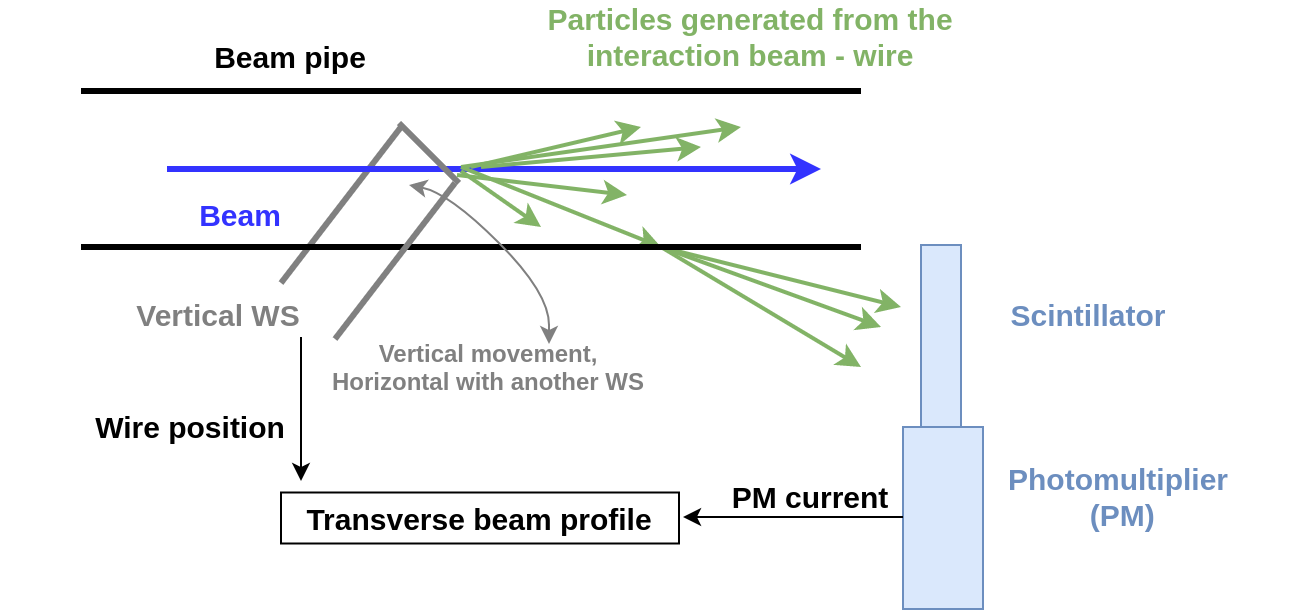
\includegraphics[width=0.8\textwidth]{images/Ch4/Wire_scanner.png}
       \caption{Sketch of the SPS rotational wire scanners~\cite{Berrig:1972478}. The wire moves across the proton beam generating secondary particles which are then detecting by a scintillator and a photomultiplier. From the measured photomultiplier current the beam profile is reconstructed.}
       \label{fig:SPS_WS_ROT}
\end{figure}

\normalsize{\textbf{Fitting of transverse profiles}}\\
Assuming gaussian beams and for $u=x,y$ being the index that respectively corresponds to the horizontal and vertical plane, the rms beam size, $\sigma_u$, is obtained following the standard procedure of least squares fitting (see Appendix~\ref{app:non_linear_fitting}). In particular, the measured beam profiles from each scan are fitted with the following four-parameter ($A, k, \mu, \sigma_u$) gaussian function:
\begin{equation}\label{eq:4p_gauss}
   f(x) = k + A e^{-\frac{(x-\mu)^2}{2 \sigma_u^2}},
\end{equation}
where $k$ is the signal offset of the PM, $A$ is the signal amplitude, $\mu$ is the mean of the Gaussian distribution and $\sigma_u$ its standard deviation. The uncertainty of the measured rms beam size, $\Delta \sigma_u$, is defined as the error of the fit of the $\sigma_u$ parameter (see Appendix~\ref{app:non_linear_fitting}).

%T A non-linear least square minimization is used to fit the gaussian function to the measured data and obtain the optimal values for the parameters ($A, k, \mu, \sigma_u$).he standard error of the parameters' estimates is given by the square root of the diagonal of their covariance matrix.~\cite{gaus_fit_least_squares}. The uncertainty of the measured beam size, $\Delta \sigma$, is defined as the standard error of the $\sigma$ parameter. The optimal parameters' values and their covariance matrix are computed here using the $\mathrm{scipy.curve \_ fit}$ \cite{scipy_curve_fit} function of Python programming language. 
% Curve fitting explanation: https://www.youtube.com/watch?v=Jl-Ye38qkRc&ab_channel=BrantCarlson

An example of the beam profile measured from the SPS WS at a specific time is shown in Fig.~\ref{fig:WS_example_V_profile} (light blue dots) along with the gaussian fit (orange line).
% Location where the figure was produced: /eos/user/n/natriant/2020/WS_analysis
\begin{figure}[!h]
   \centering         
   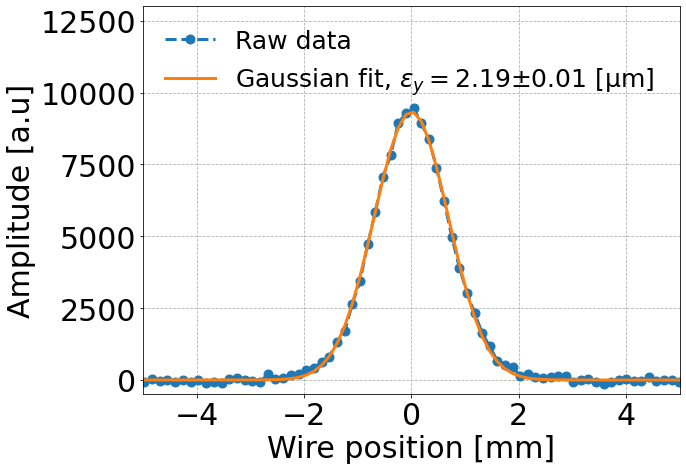
\includegraphics[width=0.6\textwidth]{images/Ch4/SPS.BWS.41677.V_ROT_2018-09-05 15_45_01.33500_raw_and_fit.png}
       \caption{Vertical beam profile obtained from the BWS.41677.V instrument. The measured data points (light blue) are fitted with a four parameter gaussian (orange) to obtain the beam size. The calculated emittance and its uncertainty are also shown.}
       \label{fig:WS_example_V_profile}
\end{figure}
   

\section{Bunch length and intensity measurements}\label{sec:bunch_length_intensity_meas_2018}

\section{Comparison of measured emittance growth with the theory}\label{sec:meas_2018_vs_theory}

Comparison of bunch 1 with theory. Discrepancy of a factor 4.
6/7 noise settings as the first noise level was found to be below the noise floor (check themis mail).

\section{Conclusions and outlook}\label{sec:MD2018_summary}





\section{SPS Wire Scanners}\label{subsec:sps_ws}




The general formula for computing the normalised beam emittance from the beam size, $\sigma$ is given by:
\begin{equation}\label{eq:emittance_from_WS}
   \centering
   \epsilon = \frac{\sigma^2}{\beta_{WS}} \betarel \gammarel ,
\end{equation}

where $\sigma$ is the rms beam size, $\beta_{WS}$ the beta function at the WS location and $\betarel, \gammarel$ the relativistic parameters.


Note that, in the 2018 SPS operational configuration, the dispersion was small at the WSs location and thus its contribution to the beam size was considered to be negligible \footnote{The dispersion at BWS.51995.H location in 2018 was $\Dx$= -15\,mm. At 270\,GeV, the energy spread, $\delta$, is of the order of $\mathrm{10^{-4}}$. Thus, from Eq.~\eqref{eq:emit_from_beam_size} the horizontal normalised emittance from the dispersion is expected at the order of $\mathrm{10^{-6} \ \mu m}$. Comparing to the observed beam size during the CC tests of a few microns the dispersion is negligible. \color{red}{The measured $\Dx, \Dy$ were found to be very small and thus their contribution is also considered negligible. The plan is to perform some measurments in 2022 to get a feeling of their values at the location of the wire scanners}}. For the $\CC$ studies at 270\,GeV beam energy, $\betarel \gammarel$ equals 287.8 and the beta functions were 81.5\,m and 62.96\,m at the locations of the horizontal and vertical WS respectively. The uncertainty on the beta functions at the location of the WS, $\Delta \beta_{WS}$, is 5$\%$ in both planes, which represents the rms beta-beating in the SPS~\cite{SPS-beta-beating-Rogelio}.
% Computations from dispersive contribution: /eos/user/n/natriant/Project_thesis/material/Ch4: 1st experimental campaign in SPS/dispersive_contribution_in_the_emittance.pdf

Assuming that the relativistic parameters are free of error, the uncertainty of the computed emittance, $\Delta \epsilon$, depends on the uncertainty of the measured beam size, $\Delta \sigma$ and of the beta function at the location of the WS, $\Delta \beta_{WS}$, as follows:

\begin{equation}\label{eq:emittance_from_WS_uncertainty}
   \centering
   \Delta \epsilon = \sqrt{\left ( \frac{\partial \epsilon}{\partial \sigma}\right )^2 \Delta \sigma^2 + \left ( \frac{\partial \epsilon}{\partial \beta_{WS}} \right )^2 \Delta \beta_{WS}^2} = \epsilon  \sqrt{\left ( \frac{2 \Delta \sigma}{\sigma}\right )^2 + \left ( \frac{ \Delta \beta_{WS}}{\beta_{WS}} \right )^2} .
\end{equation}
% Propagation of uncertainty in paper: /eos/user/n/natriant/Project_thesis/material/Ch4: 1st experimental campaign in SPS/propagation_of_uncertainty_emittance.pdf

\normalsize{\textbf{Further considerations}}\\
It is worth noting here that during each measurement with the WS the beam profile is actually acquired twice as the wire crosses the beam in the forward direction (IN scan) and then in the reverse direction (OUT scan). For the 2018 measurements the emittance values obtained from IN and OUT scans, $\epsilon_\mathrm{IN} \pm \Delta \epsilon_\mathrm{IN}$ and $\epsilon_\mathrm{OUT} \pm \Delta \epsilon_\mathrm{OUT}$, were found to be very similar. In the analysis of the 2018 measurements, the average emittance from the two scans, $\epsilon_\mathrm{avg} = \langle \epsilon_\mathrm{IN}, \epsilon_\mathrm{OUT}\rangle$, is used. The uncertainty in the average, $\Delta \epsilon_\mathrm{avg, 1}$, is given by (see Appendix ...): 
\begin{equation}\label{eq:uncertainty_mean_ws}
   \Delta \epsilon_\mathrm{avg, 1} = \frac{\mid \epsilon_\mathrm{IN} - \epsilon_\mathrm{OUT} \mid}{2 \sqrt{2}}.
\end{equation}
The propagated uncertainty from the measurement errors, $\Delta \epsilon_\mathrm{IN}$ and $\Delta \epsilon_\mathrm{OUT}$, is given by:
\begin{equation}\label{eq:propagated_uncertainty_ws}
   \Delta \epsilon_\mathrm{avg, 2} = \frac{1}{2}\sqrt{ \Delta \epsilon_\mathrm{IN}^2 + \Delta \epsilon_\mathrm{OUT}^2}.
\end{equation}
Considering that $\Delta \epsilon_\mathrm{avg, 1}$ and $\Delta \epsilon_\mathrm{avg, 2}$ are independent, the combined uncertainty in the average, $\Delta \epsilon_\mathrm{avg}$, is given by:

\begin{equation}\label{eq:combined_uncertainty_ws}
   \Delta \epsilon_\mathrm{avg} = \sqrt{\Delta \epsilon_\mathrm{avg, 1} ^2 + \Delta \epsilon_\mathrm{avg, 2} ^2}.
\end{equation}

Finally, some emittance increase is expected during each wire scan, due to multiple Coulomb scattering. This effect has been extensively studied in Ref.~\cite{Roncarolo:1481835}. For the rotational SPS WS and the energy of 270\,GeV, at which the $\CC$ experiments were performed the expected emittance growth from the WS is expected to be small. However, a conservative number of scans were carried, $\sim$ 20 scans per bunch and per plane during $\sim$ 1 hour, in order to minimise the contribution from this effect.

\section{ABWLM and Wall Current monitor}\label{sec:ABWLM_WallCurrentMonitor}

\begin{sloppypar}
The bunch length was measured with two different instruments the ABWLM (A for RF, Beam, Wideband, Longitudinal, Measurement)~\cite{ABWLM} and the Wall Current monitor~\cite{Papotti:1124099}. The ABWLM measures the longitudinal profiles from which the bunch length is computed by performing a gaussian fit. The Wall Current monitor acquirest not just the longitudinal profiles but also the longitudinal beam position relative to the monitor i.e. the beam arrival with respect to the reference. The bunch length is estimated by computing the full width half maximum of the profiles and then using it to estimate the sigma of a gaussian distribution. No further details on the operation of these instruments are discussed here as the offline analysis was not performed by the author.
\end{sloppypar}


% beam position relative to monitor
